\documentclass[conference]{IEEEtran}

% ---------------------------------------------------------------- packages
\usepackage[T1]{fontenc}
\usepackage[utf8]{inputenc}
\usepackage{cite}
\usepackage{amsmath,amssymb}
\usepackage{graphicx}
\usepackage{array}
\usepackage{booktabs}
\usepackage{multirow}
\usepackage{url}
\usepackage{xcolor}
% Clickable links: every Fig./Table/equation number and every [n] citation jumps to its target.
% Links are shown in dark blue. For black links, replace the options with [hidelinks].
\usepackage[colorlinks=true,linkcolor=blue!60!black,citecolor=blue!60!black,urlcolor=blue!60!black]{hyperref}

\graphicspath{{./}{figures/}}

% One-column figures use [H]: they appear exactly where they are written (shown first, then mentioned).
% Page-wide tables cannot be pinned in a two-column paper, so they go to the top or bottom of the
% nearest page. Their code is placed a little BEFORE the paragraph that mentions them, so they
% appear as early as possible. If a table still lands after its mention, move its block one
% paragraph further up.
\usepackage{float}       % [H] = place a one-column figure exactly here
\usepackage{stfloats}    % lets page-wide tables also go at the bottom of a page
\AtBeginDocument{\setcounter{dbltopnumber}{1}}  % at most one page-wide table at the top of each page
\raggedbottom  % do not stretch the space between paragraphs to fill a column (avoids large gaps)

\begin{document}

\title{Comparison of Classical and Diffusion-Based Image Inpainting Methods for Photo Restoration: A Pilot Study}

\author{\IEEEauthorblockN{Dilyara Kurmangazykyzy and Saule Karimova}}

\maketitle

% ---------------------------------------------------------------- abstract
\noindent{\bfseries\itshape Abstract}\par\vspace{3pt}
\noindent{\bfseries Old photographs often lose parts of the image to scratches, tears and stains, and image inpainting can restore these parts with classical or diffusion-based methods. However, the two have not been compared on damaged photographs, so it is unclear which of them restores such photographs best and fastest, and whether one of them adds details that were never in the original. The aim of this paper is therefore to compare one method based on partial differential equations, one exemplar-based method and one diffusion-based method on damaged photographs. In this pilot study, twenty photographs were covered with irregular masks imitating scratches, tears and stains over about 5\%, 20\% or 40\% of the image, and each was restored by all three methods. The restorations were compared with the originals using pixel-based and perceptual quality measures, processing time, statistical tests and visual inspection. The diffusion-based method had the lowest perceptual error in every photograph, less than half that of the classical methods at the largest damage, and needed about 0.4 seconds per image. At the largest damage, however, it replaced a person's face with another, which the quality scores did not detect. We conclude that the diffusion-based method offers the best balance between restoration quality and speed, but because it can invent convincing details, its results should be checked by a person before a restored photograph is trusted as a record of real people or events.}\par\vspace{6pt}

\noindent{\bfseries\itshape Index Terms}\par\vspace{3pt}
\noindent{\bfseries image inpainting, photo restoration, diffusion models, partial differential equations, exemplar-based inpainting, perceptual quality}\par\vspace{6pt}


% =====================================================================
\section{Introduction}
% =====================================================================

Photographs keep family memories and records of public events, but the paper prints that carry them do not last. Improper storage and environmental conditions leave scratches, folds, stains and fading on old photographs, and in severe cases whole parts of the image are lost \cite{kuo2022}. Restoring such a photograph by hand, with editing tools such as Photoshop or GIMP, depends on the skill of the person and takes a lot of time and effort \cite{kuo2022}. For this reason, damaged areas can be filled by computer using image inpainting, which reconstructs the missing parts of an image from the pixels that remain \cite{kuo2022,wang2026}.

Image inpainting is the task of reconstructing missing regions of an image from the remaining, preserved content \cite{kuo2022,wang2026}. The core challenge is that the original content of a missing area is unknown. Many different fills are possible, but only a few are consistent with the surrounding boundaries and textures \cite{wang2026}. The difficulty increases with the size of the gap, because the remaining parts of the image provide fewer clues about the lost content \cite{wang2026}. A further problem concerns authenticity, since a restoration method may generate details that look plausible but were never present in the original photograph \cite{peng2026dcadif}. For images that depict real people or events, such fabricated details are factual errors, and because the original, undamaged photograph no longer exists, the accuracy of the reconstruction cannot be verified.

Existing inpainting methods address these challenges in two ways: classical methods use only the content of the image itself, while deep-learning methods learn from large collections of images. Among the classical methods, the authors of \cite{xiao2024} proposed a partial differential equation (PDE)-based method with a P-Laplace operator that slows the spread of pixel values across sharp edges to reduce artefacts, and the authors of \cite{xie2022} improved an exemplar-based method that copies matching patches, so that the copied patches follow the lines of historic buildings. These classical methods work well on small defects, but they struggle when the missing region is large or complex. Deep-learning methods were introduced to overcome this limit; for example, the authors of \cite{wan2023} trained a network on real and synthetically damaged photographs so that it repairs scratches, dust and blur together. More recently, diffusion models, which rebuild an image by reversing a step-by-step noise process, have been shown to give a coherent overall structure \cite{wang2026}.

Diffusion models have a practical cost: one image typically needs hundreds or thousands of denoising steps, and the authors of \cite{yue2025} reduced this to as few as four by changing the noise schedule. The authors of \cite{sekrecka2025} compared classical and learning-based inpainting, but on remote sensing images rather than photographs. However, classical and diffusion-based methods have not been compared on damaged photographs, so it is unclear how much a diffusion-based method gains in quality for the time it needs. It also remains unclear whether it adds more invented details than classical methods do, a risk that matters when a photograph records real people or events.

To address this gap, we aim to compare one PDE-based, one exemplar-based and one diffusion-based inpainting method on damaged photographs. The comparison covers three things: how good the restored image is, how much time each method needs, and whether a method adds details that were never in the photograph.

Given 20 undamaged photographs from an open photograph collection, the comparison first adds an irregular mask to each photograph, covering about 5\%, 20\% or 40\% of the image. The PDE-based, exemplar-based and diffusion-based methods then each restore every damaged image with their default settings, which gives 180 restored outputs, and the two classical methods serve as the baseline for the diffusion-based method. Restoration quality is measured against the original photograph with peak signal-to-noise ratio (PSNR), structural similarity (SSIM) and learned perceptual image patch similarity (LPIPS), and processing time is recorded for each image, which covers the cost question raised above. Additionally, the restored images of one photograph of each type are compared side by side and checked by eye for artefacts and invented details. Together, these steps compare the three methods on the same photographs and masks, so that any difference in quality, time or invented content can be attributed to the method itself.

In summary, this study has three contributions. First, we compare one PDE-based, one exemplar-based and one diffusion-based method on the same 20 photographs at three damage levels. Second, we report processing time alongside PSNR, SSIM and LPIPS, so that the relationship between reconstruction quality and the time required can be evaluated. Third, we examine the restored images side by side for artefacts and invented details that numerical scores alone cannot adequately reveal.

This paper is structured as follows: Section~\ref{sec:litreview} reviews related work, and Section~\ref{sec:methods} describes the data, the three inpainting methods, the evaluation metrics and the statistical analysis. Section~\ref{sec:results} compares the restoration quality and processing time of the three methods at each damage level and shows the restored images side by side. Section~\ref{sec:discussion} discusses the results and their limitations, and Section~\ref{sec:conclusion} concludes the paper.

% =====================================================================
\section{Literature Review}
\label{sec:litreview}
% =====================================================================

Image inpainting has grown quickly, and a number of surveys now track how the field developed. A few of them cover the whole timeline, from the earliest methods to the present \cite{wang2026,jam2021}, and most concentrate on the period since around 2014, when deep neural networks began to reshape the field \cite{xiang2023,quan2024,zhang2023,xu2023,qin2021,elharrouss2025,su2022,yang2024}. These reviews group current deep-learning methods into convolutional, generative and transformer-based families, with diffusion models forming one branch of the generative family \cite{wang2026}. They also make clear that restoring a damaged photograph is more than a technical exercise. A method has to produce a convincing result without inventing details that were never there, and this matters far more for a photograph that documents a real person or event than for an ordinary test image.

Before deep learning, two families of classical methods dominated the field, and they still serve as baselines today \cite{wang2026}. PDE-based methods diffuse pixel values inward from the edge of the damaged region. A P-Laplace variant of this idea controls how fast information spreads across sharp edges compared with flat regions, which produces fewer artefacts and needs fewer iterations on images with strong noise, although it still struggles with complex or heavily textured regions \cite{xiao2024}. Exemplar-based methods instead search the undamaged part of the image for patches to copy into the hole and fill the strongest edges first \cite{wang2026}. One study adapted this priority rule to damaged historical architecture in south-eastern China, so that the copied patches followed the original building lines more closely \cite{xie2022}. Neither family needs training data, which keeps them competitive with learning-based methods on tasks where precision matters more than visual richness, such as remote sensing imagery \cite{sekrecka2025}. Both families, however, work well only on small defects and lose quality once the missing region becomes large or complex \cite{wang2026}.

Deep learning replaced these hand-crafted rules with networks that learn patterns directly from data. For old photographs, one method trains a network on a mix of real photographs and synthetically damaged pairs, so that it learns to repair scratches, dust and blur together, as they usually appear on a real photograph \cite{wan2023}. For frescoes, where training images are far scarcer than for everyday photographs, an untrained network fitted to a single damaged image was compared with hand-crafted methods on an artificial mask placed over an intact fresco \cite{merizzi2024}. Among the generative methods, diffusion models have drawn the most attention for photograph and heritage restoration. They reverse a noise-adding process step by step and use the known part of the image to guide each step, which tends to produce a coherent overall structure rather than isolated patches \cite{wang2026}. Their main cost is speed, because a single image typically needs hundreds or thousands of denoising steps. ResShift reduces this cost by restructuring the noise schedule around the residual between the damaged input and the target output, and reaches competitive quality with as few as four sampling steps \cite{yue2025}.

Heritage material has become a testing ground for diffusion-based inpainting, and recent studies adapt the general approach in different ways. One study anchors generation to the true undamaged pixels through a lossless, image-guided sampling procedure, so that mural restorations do not drift away from the original \cite{hu2025guidepaint}. Another removes roughly 83\% of the parameters of the diffusion network and uses a weighting scheme to protect fine perceptual detail, which makes mural inpainting feasible on limited computing resources \cite{zhao2026apldiff}. A third combines contour-based conditioning, a multi-scale process that moves from coarse composition to fine texture and a frequency-domain refinement step. Trained on more than 650{,}000 patches from 25 Tang-dynasty caves of the Mogao Grottoes in Dunhuang, it outperformed all ten methods it was compared with on both standard and mural-specific quality metrics \cite{han2026diffumural}. A fourth notes that structure and style can become tangled inside a single diffusion network, so that transferring style into the damaged region distorts its structure. It therefore extracts structure and style through two separate pathways and combines them with a fusion module that shifts weight from structure toward style as denoising proceeds \cite{peng2026dcadif}.

How restoration quality should be measured is not fully settled. Most studies report PSNR, which compares restored pixels directly with the original image, and SSIM, which compares structure, contrast and brightness instead of raw pixel values \cite{yang2024}. These two metrics do not always agree with what a person sees, so LPIPS compares images through the layers of a trained neural network and follows human judgement more closely \cite{yang2024}. Even LPIPS is not enough on its own. In one large study, models that scored well on these metrics were still judged implausible by 278 human experts \cite{han2026diffumural}, which shows that a good score does not guarantee a result that respects the original image. This gap between scores and perception is linked to hallucination, in which a restoration looks convincing but contains details that were never there \cite{peng2026dcadif}. For a photograph of a real person or event, such a detail is not only stylistically wrong but potentially factually wrong. Processing cost, in turn, is rarely reported alongside quality, even though it can differ greatly between methods \cite{yue2025}.

Taken together, these studies leave three gaps that matter for the present comparison. First, almost none of the heritage studies test against a classical baseline, as they compare mainly with other deep-learning methods \cite{peng2026dcadif,hu2025guidepaint,zhao2026apldiff,han2026diffumural}, and the one comparison that does include classical methods concerns remote sensing imagery rather than photographs \cite{sekrecka2025}. Second, quality is judged mostly by metric scores, although these scores can miss invented content \cite{peng2026dcadif,han2026diffumural}. Third, processing cost is seldom reported next to quality \cite{yue2025}. No study has therefore compared classical and diffusion-based methods on damaged photographs and, in the same experiment, measured their cost and checked them for invented content. This is the gap the present study addresses.

% =====================================================================
\section{Methods and Materials}
\label{sec:methods}
% =====================================================================

\subsection*{Research Design}

This study follows a controlled experimental design with two independent variables. The first is the inpainting method, which has three levels, namely a PDE-based method (Navier--Stokes, NS), an exemplar-based method (the Criminisi algorithm) and a diffusion-based method (ResShift). The two classical methods serve as baselines for the diffusion-based one. The second independent variable is the damage level, for which masks were generated to cover about 5\%, 20\% and 40\% of the image. The dependent variables are PSNR, SSIM, LPIPS and the processing time of each restored image.

To keep the comparison fair, every method restores the same photographs with exactly the same masks and at the same image size, so differences in the scores can be attributed only to the method and the amount of damage. Restoring a face is a different task from restoring a mountain, so the photographs were also balanced across three types of content, namely portraits, landscapes and group photographs. Each photograph acts as a block in the paired comparisons, and photo type is used to stratify the sample and to summarise the results separately. The runs were carried out in random order, so that the order of execution could not affect the measured times. Twenty photographs, three damage levels and three methods give 180 restored images, a sample size that suits the exploratory aim of a pilot study.

\subsection*{Data}

The twenty photographs come from the test split of BSDS500, an open collection of natural colour photographs \cite{bsds500}. We selected seven portraits of a single person with a clearly visible face, seven landscapes without people and six group photographs with at least three people, and refer to them as portrait\_1 to group\_6. The originals measure $481 \times 321$~px, or $321 \times 481$~px for upright photographs. We cropped the centre of each photograph to a square of $321 \times 321$~px and resized it to $256 \times 256$~px, the input size of the diffusion model \cite{yue2025}, and all three methods were given these resized images. The files were taken from a fixed version of the dataset and checked against their checksums, so the same twenty images can be obtained again. The dataset is publicly released for research use, and no new photographs of people were taken or collected for this study.

\subsection*{Damage Simulation}

Old photographs are damaged mainly by scratches, tears and stains \cite{kuo2022}. We imitated this damage with irregular masks rather than plain rectangles. Each mask is built from uneven strokes, which look like scratches and tears, and from blotches with jagged outlines, which look like stains, placed at random positions and with random sizes. New elements are added until the masked area is within one percentage point of 5\%, 20\% or 40\% of the image. Every photograph and damage level has its own fixed random seed, so each mask can be generated again, and the same mask is given to all three methods.

\begin{figure}[H]
  \centering
  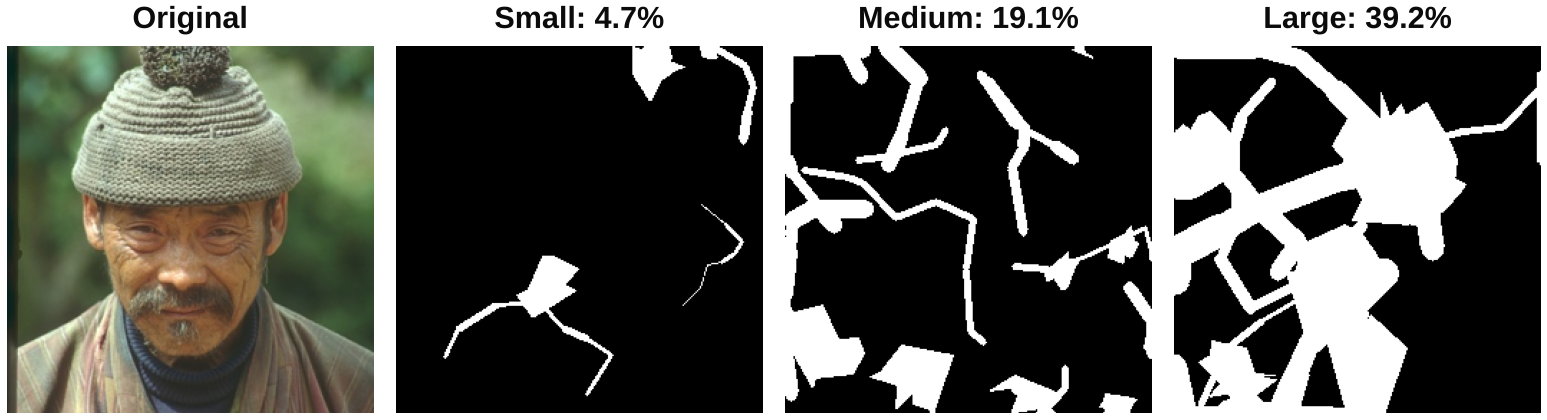
\includegraphics[width=\columnwidth]{fig1_masks.png}
  \caption{Masks at the three damage levels for one photograph (portrait\_4). White marks the damaged area, and each title gives the share of the image that is masked.}
  \label{fig:masks}
\end{figure}

Fig.~\ref{fig:masks} shows the three masks generated for one photograph. At the small level, the mask consists of a few thin strokes and two small blotches. At the medium level, the strokes are longer and wider and more blotches appear. At the large level, wide blotches join the strokes and cover large parts of the face and clothing. Across all twenty photographs, the masks covered 4.6\%, 19.7\% and 39.7\% of the image on average. In this and the following figures, the damaged area is shown in white.

\subsection*{Inpainting Methods}

The PDE-based and diffusion-based methods were run with the default settings published for them, and our implementation of the exemplar-based method follows the settings of the original algorithm, so that none of the methods received extra tuning. Each method receives the damaged image together with its mask and returns one restored image, and pixels outside the mask are never changed.

The PDE-based method fills the hole by spreading information from the surrounding pixels into it, which is the principle behind the PDE methods discussed in \cite{xiao2024}. We used the Navier--Stokes inpainting of the OpenCV library with its default radius of 3~px.

The exemplar-based method follows the Criminisi algorithm, which the method in \cite{xie2022} builds on. It fills the hole patch by patch, starting at the boundary points that have the most known pixels and the strongest edges, and for each point it copies the best-matching $9 \times 9$~px patch from the undamaged part of the image. OpenCV does not include this algorithm, so we implemented it ourselves in Python.

The diffusion-based method is ResShift \cite{yue2025}. Instead of starting from pure noise, it starts from the damaged image and shifts the residual between the damaged and the clean image, which reduces sampling to four steps. We used the pretrained inpainting model released by its authors.

\subsection*{Evaluation Metrics}

We evaluate each restored image with three quality measures and its processing time \cite{yang2024}. PSNR measures the pixel-wise difference between the restored and the original image,
\begin{equation}
  \mathrm{PSNR} = 10 \cdot \log_{10}\left(\frac{\mathrm{MAX}_I^2}{\mathrm{MSE}}\right),
  \label{eq:psnr}
\end{equation}
where $\mathrm{MAX}_I$ is the maximum possible pixel value and MSE is the mean squared error between the two images. SSIM compares local brightness, contrast and structure,
\begin{equation}
  \mathrm{SSIM}(x,y) = \frac{(2\mu_x\mu_y + C_1)(2\sigma_{xy} + C_2)}{(\mu_x^2 + \mu_y^2 + C_1)(\sigma_x^2 + \sigma_y^2 + C_2)},
  \label{eq:ssim}
\end{equation}
where $\mu$ and $\sigma$ are the local mean and standard deviation of an image patch and $\sigma_{xy}$ is the covariance between the two patches. LPIPS compares the two images through the features of a pretrained network, which brings it closer to human judgement \cite{yang2024},
\begin{equation}
  \mathrm{LPIPS}(x,y) = \sum_{l} \frac{1}{H_l W_l} \sum_{h,w} \left\lVert \phi_l(x)_{hw} - \phi_l(y)_{hw} \right\rVert_2^2,
  \label{eq:lpips}
\end{equation}
where $\phi_l$ are the activations of layer $l$ and $H_l$ and $W_l$ are its height and width. We used the standard LPIPS model based on the AlexNet network. A higher PSNR and SSIM and a lower LPIPS mean that the restoration is closer to the original.

All scores are computed on the full $256 \times 256$~px image, because this is the image a viewer sees after restoration. Pixels outside the mask are identical for all three methods, so they raise PSNR and SSIM for every method and make the differences between methods smaller than they would be inside the masked area alone. Processing time is the time in seconds from input to output for one image with the implementations described above, and loading the diffusion model once before the experiment is not included. For each method and damage level we report the mean and standard deviation over the twenty photographs. Invented details cannot be captured by these scores, so we also compare the restorations of one photograph of each type side by side and inspect them by eye for blur, misplaced patches and content that is not present in the original.

\subsection*{Statistical Analysis}

To compare the methods statistically, we start from the assumption that the three methods perform equally at a given damage level. The tests first check whether the scores give enough evidence against this assumption and, if they do, which of the methods differ from each other. Every method restored the same photographs, so the scores of the three methods are paired, and we therefore use tests for paired data, following \cite{chung2026} and \cite{rainio2024}.

The first step is a Friedman test for each measure and damage level. Within each photograph, the three methods are ranked from 1 to 3 on the measure in question, and the test statistic is
\begin{equation}
  \chi^2_F = \frac{12}{n k (k+1)} \sum_{j=1}^{k} R_j^2 - 3n(k+1),
  \label{eq:friedman}
\end{equation}
where $n = 20$ is the number of photographs, $k = 3$ is the number of methods and $R_j$ is the sum of the ranks of method $j$ over all photographs. If the three methods performed equally, $\chi^2_F$ would follow a chi-square distribution with $k - 1 = 2$ degrees of freedom. Its largest possible value, $n(k - 1) = 40$, is reached when the three methods are ranked in the same order in every photograph.

When the Friedman test shows a difference, the second step finds where it lies. Processing time is treated as a cost rather than a quality measure, so it is tested with the Friedman test alone. For each quality measure, we compared the diffusion-based method with each baseline, and the two baselines with each other, using the Wilcoxon signed-rank test. For every photograph $i$, the difference $d_i$ between the scores of the two methods is computed, the absolute differences are ranked, and the statistic is the sum of the ranks of the positive differences,
\begin{equation}
  W^{+} = \sum_{i \,:\, d_i > 0} \operatorname{rank}\left(|d_i|\right).
  \label{eq:wilcoxon}
\end{equation}

If neither method is better, $W^{+}$ stays close to its expected value $n(n + 1)/4 = 105$, and a value far from it shows that one method scores better in most photographs. Each measure and damage level involves $m = 3$ such comparisons, and the p-values within each of these sets are adjusted with Holm's correction. The correction is not applied across measures or damage levels, which is acceptable for an exploratory study. The p-values are sorted in ascending order, $p_{(1)} \le p_{(2)} \le p_{(3)}$, and each is replaced by
\begin{equation}
  p^{\mathrm{Holm}}_{(i)} = \max_{j \le i} \, \min\left\{1,\; (m - j + 1)\, p_{(j)}\right\}.
  \label{eq:holm}
\end{equation}

A corrected p-value below 0.05 is taken as significant. Twenty photographs form a small sample, so we treat these tests as exploratory. To make the comparison easier to follow, we also count in how many of the twenty photographs the diffusion-based method scored better than each baseline. Finally, the mean scores were summarised separately for portraits, landscapes and group photographs, to check whether the ranking depends on image content.

% =====================================================================
\section{Results}
\label{sec:results}
% =====================================================================

All 180 restorations were scored against their undamaged originals, and two patterns run through the results. The quality of every method fell steadily as more of the image was missing. At the same time, the diffusion-based method kept a clear lead on the perceptual measure, LPIPS, and stayed close to the PDE-based method on the pixel-based measures, PSNR and SSIM. In what follows, we first show this pattern in the scores, test whether it holds across individual photographs and check whether it depends on photo type. We then turn to processing time and, finally, to the restored images themselves.

\begin{table*}[!b]
  \centering
  \renewcommand{\arraystretch}{1.15}
  \begin{tabular}{llcccc}
    \toprule
    Damage & Method & PSNR (dB) $\uparrow$ & SSIM $\uparrow$ & LPIPS $\downarrow$ & Time (s) $\downarrow$ \\
    \midrule
    \multirow{3}{*}{Small ($\approx$5\%)}
      & PDE-based       & 35.33 $\pm$ 3.36 & \textbf{0.9813 $\pm$ 0.0059} & 0.0157 $\pm$ 0.0081 & \textbf{0.005 $\pm$ 0.001} \\
      & Exemplar-based  & 32.34 $\pm$ 3.75 & 0.9709 $\pm$ 0.0065 & 0.0206 $\pm$ 0.0073 & 3.260 $\pm$ 0.360 \\
      & Diffusion-based & \textbf{35.43 $\pm$ 3.21} & 0.9804 $\pm$ 0.0063 & \textbf{0.0095 $\pm$ 0.0044} & 0.388 $\pm$ 0.016 \\
    \midrule
    \multirow{3}{*}{Medium ($\approx$20\%)}
      & PDE-based       & 26.60 $\pm$ 2.84 & 0.9072 $\pm$ 0.0171 & 0.0891 $\pm$ 0.0244 & \textbf{0.020 $\pm$ 0.003} \\
      & Exemplar-based  & 23.88 $\pm$ 3.06 & 0.8643 $\pm$ 0.0221 & 0.0973 $\pm$ 0.0245 & 13.318 $\pm$ 0.399 \\
      & Diffusion-based & \textbf{26.86 $\pm$ 2.43} & \textbf{0.9084 $\pm$ 0.0205} & \textbf{0.0430 $\pm$ 0.0108} & 0.384 $\pm$ 0.021 \\
    \midrule
    \multirow{3}{*}{Large ($\approx$40\%)}
      & PDE-based       & 21.94 $\pm$ 2.43 & 0.7867 $\pm$ 0.0472 & 0.2156 $\pm$ 0.0640 & \textbf{0.035 $\pm$ 0.003} \\
      & Exemplar-based  & 19.70 $\pm$ 2.75 & 0.7070 $\pm$ 0.0418 & 0.2280 $\pm$ 0.0340 & 25.606 $\pm$ 0.976 \\
      & Diffusion-based & \textbf{22.54 $\pm$ 2.75} & \textbf{0.7900 $\pm$ 0.0521} & \textbf{0.1025 $\pm$ 0.0288} & 0.383 $\pm$ 0.020 \\
    \bottomrule
  \end{tabular}
  \vspace{4pt}
  \caption{Restoration quality and processing time of the three methods at each damage level (mean $\pm$ SD, $n = 20$ photographs per row). The best value at each damage level is shown in bold.}
  \label{tab:main}
\end{table*}

\begin{table*}[!b]
  \centering
  \renewcommand{\arraystretch}{1.15}
  \begin{tabular}{llcccccc}
    \toprule
    & & \multicolumn{3}{c}{vs PDE-based} & \multicolumn{3}{c}{vs exemplar-based} \\
    \cmidrule(lr){3-5} \cmidrule(lr){6-8}
    Measure & Damage & Difference & Better & $p$ & Difference & Better & $p$ \\
    \midrule
    \multirow{3}{*}{PSNR (dB)}
      & Small  & $+0.10$ & 11/20 & .729 & $+3.09$ & 20/20 & $<$ .001 \\
      & Medium & $+0.26$ & 10/20 & .648 & $+2.99$ & 20/20 & $<$ .001 \\
      & Large  & $+0.60$ & 13/20 & .030 & $+2.84$ & 20/20 & $<$ .001 \\
    \midrule
    \multirow{3}{*}{SSIM}
      & Small  & $-0.0009$ & 6/20  & .097 & $+0.0095$ & 20/20 & $<$ .001 \\
      & Medium & $+0.0012$ & 11/20 & .674 & $+0.0440$ & 20/20 & $<$ .001 \\
      & Large  & $+0.0032$ & 10/20 & .409 & $+0.0830$ & 20/20 & $<$ .001 \\
    \midrule
    \multirow{3}{*}{LPIPS}
      & Small  & $-0.0062$ & 20/20 & $<$ .001 & $-0.0111$ & 20/20 & $<$ .001 \\
      & Medium & $-0.0461$ & 20/20 & $<$ .001 & $-0.0543$ & 20/20 & $<$ .001 \\
      & Large  & $-0.1131$ & 20/20 & $<$ .001 & $-0.1256$ & 20/20 & $<$ .001 \\
    \bottomrule
  \end{tabular}
  \vspace{4pt}
  \caption{The diffusion-based method compared with each baseline. Difference = diffusion-based minus baseline. Better = number of photographs (out of 20) in which the diffusion-based method scored better. $p$ = Holm-corrected Wilcoxon signed-rank test.}
  \label{tab:pairwise}
\end{table*}

\begin{table*}[!t]
  \centering
  \small
  \setlength{\tabcolsep}{4pt}
  \renewcommand{\arraystretch}{1.15}
  \begin{tabular}{llccccccccc}
    \toprule
    & & \multicolumn{3}{c}{PSNR (dB) $\uparrow$} & \multicolumn{3}{c}{SSIM $\uparrow$} & \multicolumn{3}{c}{LPIPS $\downarrow$} \\
    \cmidrule(lr){3-5} \cmidrule(lr){6-8} \cmidrule(lr){9-11}
    Type & Damage & PDE & Exemplar & Diffusion & PDE & Exemplar & Diffusion & PDE & Exemplar & Diffusion \\
    \midrule
    \multirow{3}{*}{Portrait}
      & Small  & 35.12 & 31.54 & \textbf{35.58} & 0.9830 & 0.9707 & \textbf{0.9834} & 0.0112 & 0.0218 & \textbf{0.0074} \\
      & Medium & 26.43 & 23.95 & \textbf{27.10} & 0.9080 & 0.8667 & \textbf{0.9127} & 0.0820 & 0.0980 & \textbf{0.0378} \\
      & Large  & 21.69 & 19.92 & \textbf{22.33} & 0.7935 & 0.7120 & \textbf{0.8019} & 0.1972 & 0.2298 & \textbf{0.0936} \\
    \midrule
    \multirow{3}{*}{Landscape}
      & Small  & \textbf{36.40} & 34.24 & 36.09 & \textbf{0.9793} & 0.9711 & 0.9767 & 0.0212 & 0.0189 & \textbf{0.0114} \\
      & Medium & \textbf{27.58} & 24.78 & 27.29 & \textbf{0.9017} & 0.8642 & 0.8960 & 0.1109 & 0.0918 & \textbf{0.0498} \\
      & Large  & 22.85 & 20.67 & \textbf{23.37} & \textbf{0.7761} & 0.7090 & 0.7701 & 0.2674 & 0.2170 & \textbf{0.1145} \\
    \midrule
    \multirow{3}{*}{Group}
      & Small  & 34.32 & 31.05 & \textbf{34.49} & \textbf{0.9815} & 0.9708 & 0.9812 & 0.0145 & 0.0212 & \textbf{0.0098} \\
      & Medium & 25.65 & 22.74 & \textbf{26.08} & 0.9127 & 0.8618 & \textbf{0.9177} & 0.0720 & 0.1028 & \textbf{0.0412} \\
      & Large  & 21.16 & 18.30 & \textbf{21.82} & 0.7912 & 0.6987 & \textbf{0.7993} & 0.1765 & 0.2389 & \textbf{0.0988} \\
    \bottomrule
  \end{tabular}
  \vspace{4pt}
  \caption{Mean PSNR (dB), SSIM and LPIPS of the three methods for each photo type and damage level (7 portraits, 7 landscapes and 6 group photographs). The best value of each measure in each row is shown in bold.}
  \label{tab:types}
\end{table*}

\subsection*{Restoration Quality}

\begin{figure}[H]
  \centering
  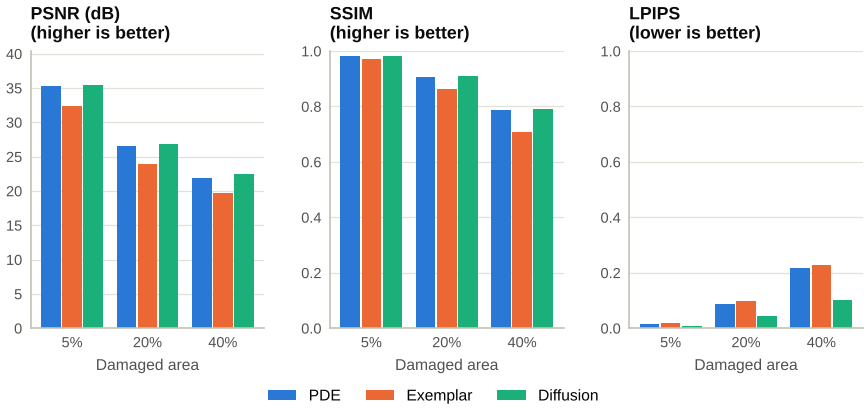
\includegraphics[width=\columnwidth]{fig2_quality.png}
  \caption{Mean PSNR, SSIM and LPIPS of the three methods at each damage level ($n = 20$ photographs). SSIM and LPIPS are shown on a common 0--1 axis.}
  \label{fig:quality}
\end{figure}

Fig.~\ref{fig:quality} gives an overview of the three quality measures. The PSNR and SSIM bars of the PDE-based and diffusion-based methods are almost the same height at every damage level, and the exemplar-based method is the lowest on both. The LPIPS bars tell a different story. They rise for all three methods as the damage increases, but those of the diffusion-based method rise much more slowly, and at the large damage level they reach less than half the height of the other two.

Table~\ref{tab:main} lists the exact values behind these bars. From the small level, where on average 4.6\% of the image was masked, to the large level, where 39.7\% was masked, PSNR fell by 12.6 to 13.4~dB for every method, so the amount of damage affected all three methods in a similar way. With small damage, the PDE-based and diffusion-based methods are almost tied on PSNR and SSIM, the exemplar-based method is about 3~dB lower on PSNR, and only LPIPS separates the methods clearly.

As the damage grows, the measures start to disagree. At the medium and large levels, the PDE-based and diffusion-based methods stay within 0.6~dB of each other on PSNR and within 0.004 on SSIM. LPIPS, however, separates them strongly. At the large level the LPIPS of the diffusion-based method is 0.103, less than half of the 0.216 of the PDE-based and the 0.228 of the exemplar-based method. On the pixel-based measures, the exemplar-based method falls furthest behind at every level.

Whether these differences hold across individual photographs is tested in Table~\ref{tab:pairwise}. The Friedman test first confirmed that the three methods differ on all three measures at every damage level ($\chi^2_F = 28.3$--$31.6$, $p < .001$), so the assumption that the methods perform equally was rejected in every case. Against the exemplar-based method, the diffusion-based method scored better on every measure in all twenty photographs. Against the PDE-based method, the outcome depends on the measure. On LPIPS, the diffusion-based method was again better in all twenty photographs at every level. On SSIM, none of the differences was significant, and on PSNR only the 0.60~dB difference at the large level reached significance (13 of 20 photographs, $p = .030$).

Between the two baselines, the PDE-based method reached a higher PSNR and SSIM than the exemplar-based method at every damage level ($p < .001$). On LPIPS, the two baselines differed significantly only at the small level ($p = .036$).

Table~\ref{tab:types} repeats this comparison for each photo type, and the same ranking appears in all three. In portraits, landscapes and group photographs alike, the diffusion-based method had the lowest LPIPS and the exemplar-based method the lowest PSNR and SSIM at every damage level. Group photographs were the hardest to restore and gave the lowest PSNR of the three types for every method, between 18.30 and 21.82~dB at the large level. Landscapes showed the only reversals. There, the PDE-based method had a slightly higher SSIM than the diffusion-based method at every level and a slightly higher PSNR at the small and medium levels, and the exemplar-based method had a lower LPIPS than the PDE-based method.

\subsection*{Processing Time}

The last column of Table~\ref{tab:main} shows that, with the implementations used here, the methods differ far more in cost than in quality. The PDE-based method needed only 0.005 to 0.035~s per image. The diffusion-based method took about 0.38~s, and this time did not change with the damage level. The exemplar-based method was the only one whose time grew with the damage, from 3.26~s at the small level to 13.32~s at the medium level and 25.61~s at the large level, which is about 67 times the time of the diffusion-based method. At every damage level, the order of the three methods was the same in every photograph ($\chi^2_F = 40.0$, $p < .001$), which is the largest value the Friedman statistic can take with twenty photographs.

\subsection*{Visual Comparison}

The scores summarise restoration quality in numbers, but they cannot show what kind of errors each method makes. We therefore look at the restored images directly, using the first photograph of each type, portrait\_1, landscape\_1 and group\_1, which were fixed in advance rather than chosen for their scores.

\begin{figure}[H]
  \centering
  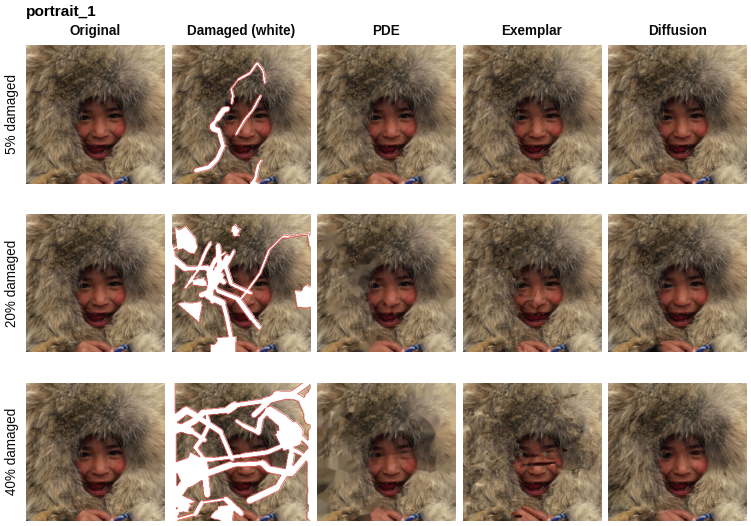
\includegraphics[width=\columnwidth]{fig3_portrait1.png}
  \caption{Restorations of portrait\_1 at the three damage levels. The damaged area is shown in white.}
  \label{fig:portrait}
\end{figure}

Fig.~\ref{fig:portrait} shows how the restorations change with the amount of damage. At the small level, all three results are hard to tell apart from the original. At the medium level, the PDE-based method begins to leave smooth, smeared patches in the fur, and the exemplar-based method leaves small dark specks around the mouth. At the large level these problems become obvious. The PDE-based result is blurred over large parts of the hood, and the exemplar-based result has a dark band across the eyes and mouth. The diffusion-based method keeps the texture of the fur and the shape of the face at all three levels.

\begin{figure}[H]
  \centering
  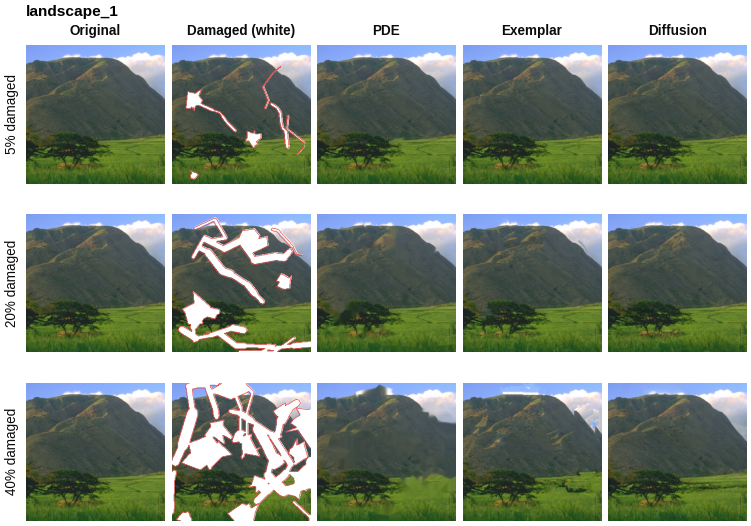
\includegraphics[width=\columnwidth]{fig4_landscape1.png}
  \caption{Restorations of landscape\_1 at the three damage levels. The damaged area is shown in white.}
  \label{fig:landscape}
\end{figure}

The landscape in Fig.~\ref{fig:landscape} belongs to the photo type in which the classical methods came closest to the diffusion-based method. At the small level, the three results can hardly be told apart from the original. At the medium level, the PDE-based method leaves a few soft, blurred patches on the slope and around the tree, and the exemplar-based method pastes a streak of cloud onto the edge of the mountain. At the large level, the PDE-based method turns parts of the slope and the grass into flat, smeared areas, and the exemplar-based method copies fragments of sky and cloud into the ridge. The diffusion-based method restores a continuous ridge line and a natural texture on the slope and in the grass.

\begin{figure}[H]
  \centering
  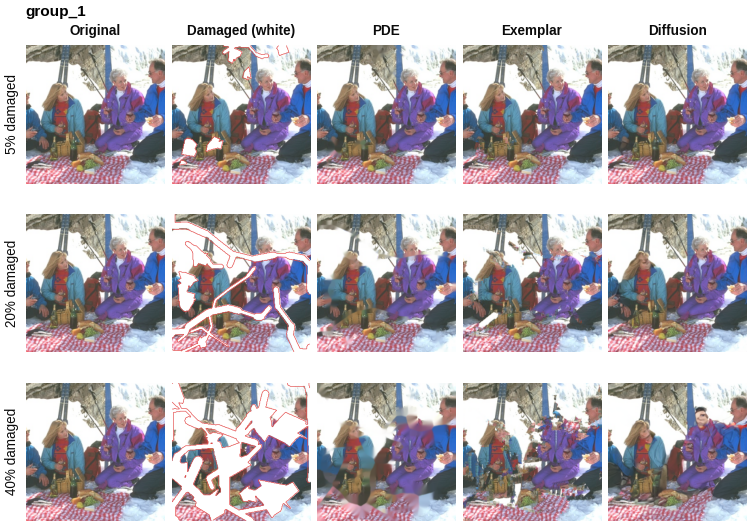
\includegraphics[width=\columnwidth]{fig5_group1.png}
  \caption{Restorations of group\_1 at the three damage levels. The damaged area is shown in white.}
  \label{fig:group}
\end{figure}

The group photograph in Fig.~\ref{fig:group} follows the same trend up to the medium level, where all three methods keep the people recognisable. At the large level, the PDE-based method blurs the centre of the picture and the exemplar-based method fills it with fragments of clothing. The diffusion-based method again produces the most plausible-looking image, but the white-haired woman in the centre is no longer there. In her place, the model has painted a different person with dark hair, whose face does not exist in the original photograph.

% =====================================================================
\section{Discussion}
\label{sec:discussion}
% =====================================================================

\subsection*{Interpretation of the Results}

The most striking result is the gap between the pixel-based measures and LPIPS. The PDE-based and diffusion-based methods are almost tied on PSNR and SSIM, yet LPIPS clearly favours the diffusion-based method, and at the large damage level its perceptual distance is less than half that of the PDE-based method. The reason lies in what each measure rewards. PSNR and SSIM compare images pixel by pixel or patch by patch, so a smooth average such as the fill of the PDE-based method keeps the error low even though it looks blurred, as Fig.~\ref{fig:portrait} shows. The diffusion-based method instead generates texture that looks like fur, hair or grass but does not match the original pixel for pixel, and the pixel-based measures give it little credit for that. Because the scores are computed on the full image, the unchanged pixels outside the mask narrow these gaps further. LPIPS compares images through the features of a trained network, so it penalises blur and rewards realistic texture. This agrees with earlier work showing that LPIPS follows human judgement more closely than PSNR and SSIM \cite{yang2024} and that good metric scores do not guarantee a result that people find plausible \cite{han2026diffumural}. The exemplar-based method copies whole patches from elsewhere in the image. When a patch does not fit, as on the face in Fig.~\ref{fig:portrait}, it breaks edges and structures, and all three measures penalise it.

The small reversals for landscapes fit the same explanation. Grass, water and foliage are repeating textures, so a patch copied from another part of the image often fits, and a smooth fill looks less wrong on a sky or a meadow than on a face. Portraits and group photographs contain structures that appear only once, such as eyes and mouths, which neither a blur nor a copied patch can reproduce. Group photographs combine several small faces in one image and were therefore the hardest case for every method.

The processing times follow from how the methods work, although their exact values also depend on the implementations. The exemplar-based method searches the whole undamaged image for every patch it fills, so the more damage there is, the longer it takes. The diffusion-based method always performs the same four sampling steps, whatever the size of the hole. This short sampling is the main idea of ResShift \cite{yue2025}. Earlier diffusion-based inpainting methods need hundreds of steps and name slow sampling as their main limitation \cite{lugmayr2022repaint}, so a diffusion model without this design would likely have been far slower. The PDE-based method only solves an equation around the damaged pixels and stays the fastest at every damage level.

The replaced face in Fig.~\ref{fig:group} shows the price of this realism. A generative model fills a hole with what is likely given the images it was trained on, not with what was actually there. When most of a face is hidden, the most likely completion can be a convincing face of somebody else. The same risk has been reported for diffusion-based restoration of murals \cite{peng2026dcadif}, and RePaint observed that diffusion models can fill very large holes with realistic content that differs strongly from the original \cite{lugmayr2022repaint}. Our scores did not reveal this error. The diffusion-based method still had the best mean LPIPS for group photographs, so a good perceptual score says nothing about whether the restored content is true.

Inpainting studies often compare methods only by their average scores, as in \cite{jiang2025,sumathi2024}. The paired tests in this study show why this can mislead. The small PSNR lead of the diffusion-based method over the PDE-based method at the small and medium levels, between 0.1 and 0.3~dB on average, was not consistent across photographs. The LPIPS advantage, by contrast, held in every single photograph. Testing paired scores, as recommended in \cite{rainio2024} and done in \cite{chung2026}, therefore separates consistent differences from accidental ones.

\subsection*{Practical Implications}

For anyone restoring a damaged photograph, these results suggest a simple rule. When the damage is small, the PDE-based method is a sensible choice, because its results are almost as good as those of the diffusion-based method and it needs only milliseconds. When larger parts are missing, the diffusion-based method produces restorations with a much lower perceptual distance and fewer visible artefacts, in less than half a second per image. Its results should, however, be checked by a person, especially when a photograph shows real people or events, because an invented face looks just as convincing as a real one. The exemplar-based implementation tested here was both the slowest and the least accurate of the three and is hard to recommend for photographs.

\subsection*{Limitations}

Several limitations should be kept in mind when reading these results. First, the damage was simulated. Our masks imitate scratches, tears and stains, but real damage also includes fading, colour shifts and missing corners, which may affect the methods differently. Second, the photographs are modern colour images rather than scanned old prints, and they were reduced to $256 \times 256$~px, so larger images may change both the quality and the processing time of each method. Third, each family of methods was represented by a single method with its default settings, and the diffusion-based method was run with one random seed. Other diffusion models and other deep learning approaches were not tested, so our conclusions apply to ResShift rather than to diffusion-based inpainting in general. Fourth, all scores were computed on the full image, and the pixels outside the mask, which are the same for every method, make the differences between methods look smaller than they are inside the damaged area. Fifth, invented details were judged only by eye on three examples, without a numerical measure or independent observers. Sixth, the processing times depend on the implementations. The PDE-based method runs in the optimised OpenCV library, and our exemplar-based implementation is plain Python code, so its times reflect the implementation as much as the algorithm. Finally, twenty photographs form a small sample, and the statistical tests should be read as exploratory. A follow-up study could address most of these points by using scanned damaged photographs at full resolution, several methods per family, scores computed inside the masked area and ratings from human observers.

% =====================================================================
\section{Conclusion}
\label{sec:conclusion}
% =====================================================================

This pilot study compared a PDE-based (NS), an exemplar-based (Criminisi) and a diffusion-based (ResShift) inpainting method on twenty photographs with three levels of simulated damage. The diffusion-based method had the lowest LPIPS in every photograph and at every damage level and gave the most plausible results in visual inspection, although its PSNR and SSIM were close to those of the PDE-based method. With the implementations used here, the PDE-based method was the fastest, the diffusion-based method needed less than half a second per image, and the exemplar-based method was both the slowest and the least accurate. At large damage, the diffusion-based method also invented content and replaced a person's face in one photograph, which the average scores did not reveal. In this pilot study, the diffusion-based method therefore offered the best balance between quality and time, provided that its results are checked by a person. Future work should test more methods on real damaged photographs, compute the scores inside the damaged area and include human judgements of authenticity.

\section*{Use of AI Tools}

An AI assistant (Claude, Anthropic) was used to help write the experiment code and to edit the language of this manuscript. The experiments were run by the authors, and the authors checked all text, numbers and references.

% ---------------------------------------------------------------- references
\bibliographystyle{IEEEtran}
\bibliography{references}

\end{document}
